\section{GPU-Accelerated Octree Encoding/Decoding}\label{sec:gpu-octree}

%\textbf{Page budget: 3 pages?}

%% \begin{outline}

%%   Background (about 1 column)
%%   \begin{itemize}
%%   \item Voxelization \status{[Done]}
%%   \item Octree basics: also describe Octree coding \status{[Done]}
%%   \item RAHT algorithm \status{[Done]}
%%   \item Entropy coding \status{[Done]}
%%   \end{itemize}

%%   \eduardo{there are various resolution levels 3DGS encoder: voxelization, geometry octree coding, attribute transforms, attribute RLGR. 3DGS decoder: attribute inverse RLGR, geometry octree decoding, attribute inverse RAHT. For this 3DGS encoder and decoder, there are dependencies (e.g., need to do voxelization first), for decoder need to decode geometry first before inverse raht, but octree decoding can be parallel with RLGR decoding. Then there is the second level of parallelization, which is  parallel RAHT/inverseRAHT, prelude, RLGR, octree coding/decoding.}

%%   Octree coding: (sub-section, about 2 pages) \status{[Done]}
%%   \begin{itemize}
%%   \item Describe standard octree encoding algorithm (tree construction, bitstream generation) (sequential version); make the point here that this needs a voxelized representation (we do this in the GPU) \status{[Done]}
%%   \item Show a table of quote/approaches from related work about how difficult it is parallelize this. \status{[Done]}
%%   \item Before explaining our idea: describe morton code \status{[Done]}
%%   \item Key idea: morton code enables $O(1)$ parent-child determination (show using a figure) \status{[Done]}
%%   \item How to parallelize Octree encoding: \status{[Done]}
%%     \begin{itemize}
%%     \item Tree construction: show by example; \status{[Done]}
%%     \item Bitstream construction: show by example \status{[Done]}
%%     \end{itemize}
%%   \item Detailed algorithm with listing and discussion of the algorithm \status{[Done]}
%%     \begin{itemize}
%%     \item But when you describe this, organize it in a template so that for subsequent algorithms, all that needs to change is the code/steps executed at each node/at each level of the parallelism \status{[Done]}
%%     \end{itemize}
%%   \end{itemize}

%%   RAHT prelude and encoding (about a page) \status{[Done]}
%%   \begin{itemize}
%%     \item Show a simple example for what the prelude and encoding do
%%     \item Describe the detailed algorithms using the template discussed above.
%%       \begin{itemize}
%%       \item Describe inputs and outputs
%%       \end{itemize}
%%   \end{itemize}

%%   Quantization (half a column) \status{[Done]}
%%   \begin{itemize}
%%   \item Background: on what quantization is and how it relates to quality
%%   \item Briefly describe how we do quantization
%%   \end{itemize}

%%   Entropy coding (half a column) \status{[Done]}
%%   \begin{itemize}
%%   \item Describe inputs and outputs
%%   \item Describe how we do RLGR parallelism: block-based to leverage GPU cores
%%   \end{itemize}

%%   Decoding: \status{[Done]}
%%   \begin{itemize}
%%   \item Explain that this is the reverse
%%   \item Describe what metadata the encoder needs to send
%%   \end{itemize}
      
%% \end{outline}

We first describe our GPU-accelerated octree encoding algorithm, which encodes Gaussian position attributes efficiently.

\subsection{Background}\label{sec:background}

\parab{Voxelization.}
%
Gaussians can be positioned irregularly in space, and all 3-D compression algorithms first \textit{voxelize} Gaussian positions to regularize the data.
%
Voxelization discretizes the cuboid bounding all the Gaussians into a regular grid of $2^J \times 2^J \times 2^J$ cubes, where $J$ is a voxelization parameter which controls the \textit{resolution} of the \gs{} frame.
%
Then, it maps each Gaussian's 3-D position to one of the cubes, by quantizing the position coordinates to use $J$ bits.
%
Multiple Gaussians might fall into a single voxel; \gsnfs{} replaces those Gaussians with a single Gaussian whose position is at the center of the voxel and other attributes are the average of the original Gaussians.\footnote{This may not be ideal for small $J$, but suffices for the range of $J$ we consider in this paper.}

%% \ao{Depending on the choice of J, averaging may not be ideal, especially if J is small. If we mostly operate in a high J setting, this may not be a problem. }

%% discretizes space into cubes, where each cube is called a \textit{voxel}.
%% %
%% For a set of $N$ Gaussians in a \gs frame with 3D positions $V = [v_i \in \mathbb{R}^3]_{i=1}^N$.
%% %
%% First, we voxelize the 3D space into a regular grid of dimension $2^J \times 2^J \times 2^J$ and map each Gaussian to an integer voxel of unit cube size where the voxel center has coordinate $\hat{v}_i \in \{0, \dots, 2^J-1\}^3$; $0$ and $2^J-1$ represents the minimum and maximum coordinate of a tight bounding box of the \gs model, respectively.
%% %
%% Since multiple Gaussians can fall into the same voxel, we merge them by averaging their attributes.

%% In the process of voxelization, the points are partitioned into voxels, and the attributes associated with the 3D points in a voxel are aggregated.
%% %
%% Voxelization is often used as a preprocessing step for 3D compression algorithms, as it provides a structured format that can be efficiently encoded.

%% %
%% Both voxelization and merging can be parallelized on GPU by launching one thread per Gaussian, which computes the voxel coordinate and atomically accumulates the attributes into the corresponding voxel.
%% %
%% This process reduces the number of Gaussians and improves compressibility. The voxelized \gs model has $\hat{N}_v$ unique gaussians, where position of each gaussian lies exclusively at the center of a voxel with its averaged attribute.

% \begin{figure}[t]
%   \centering
%   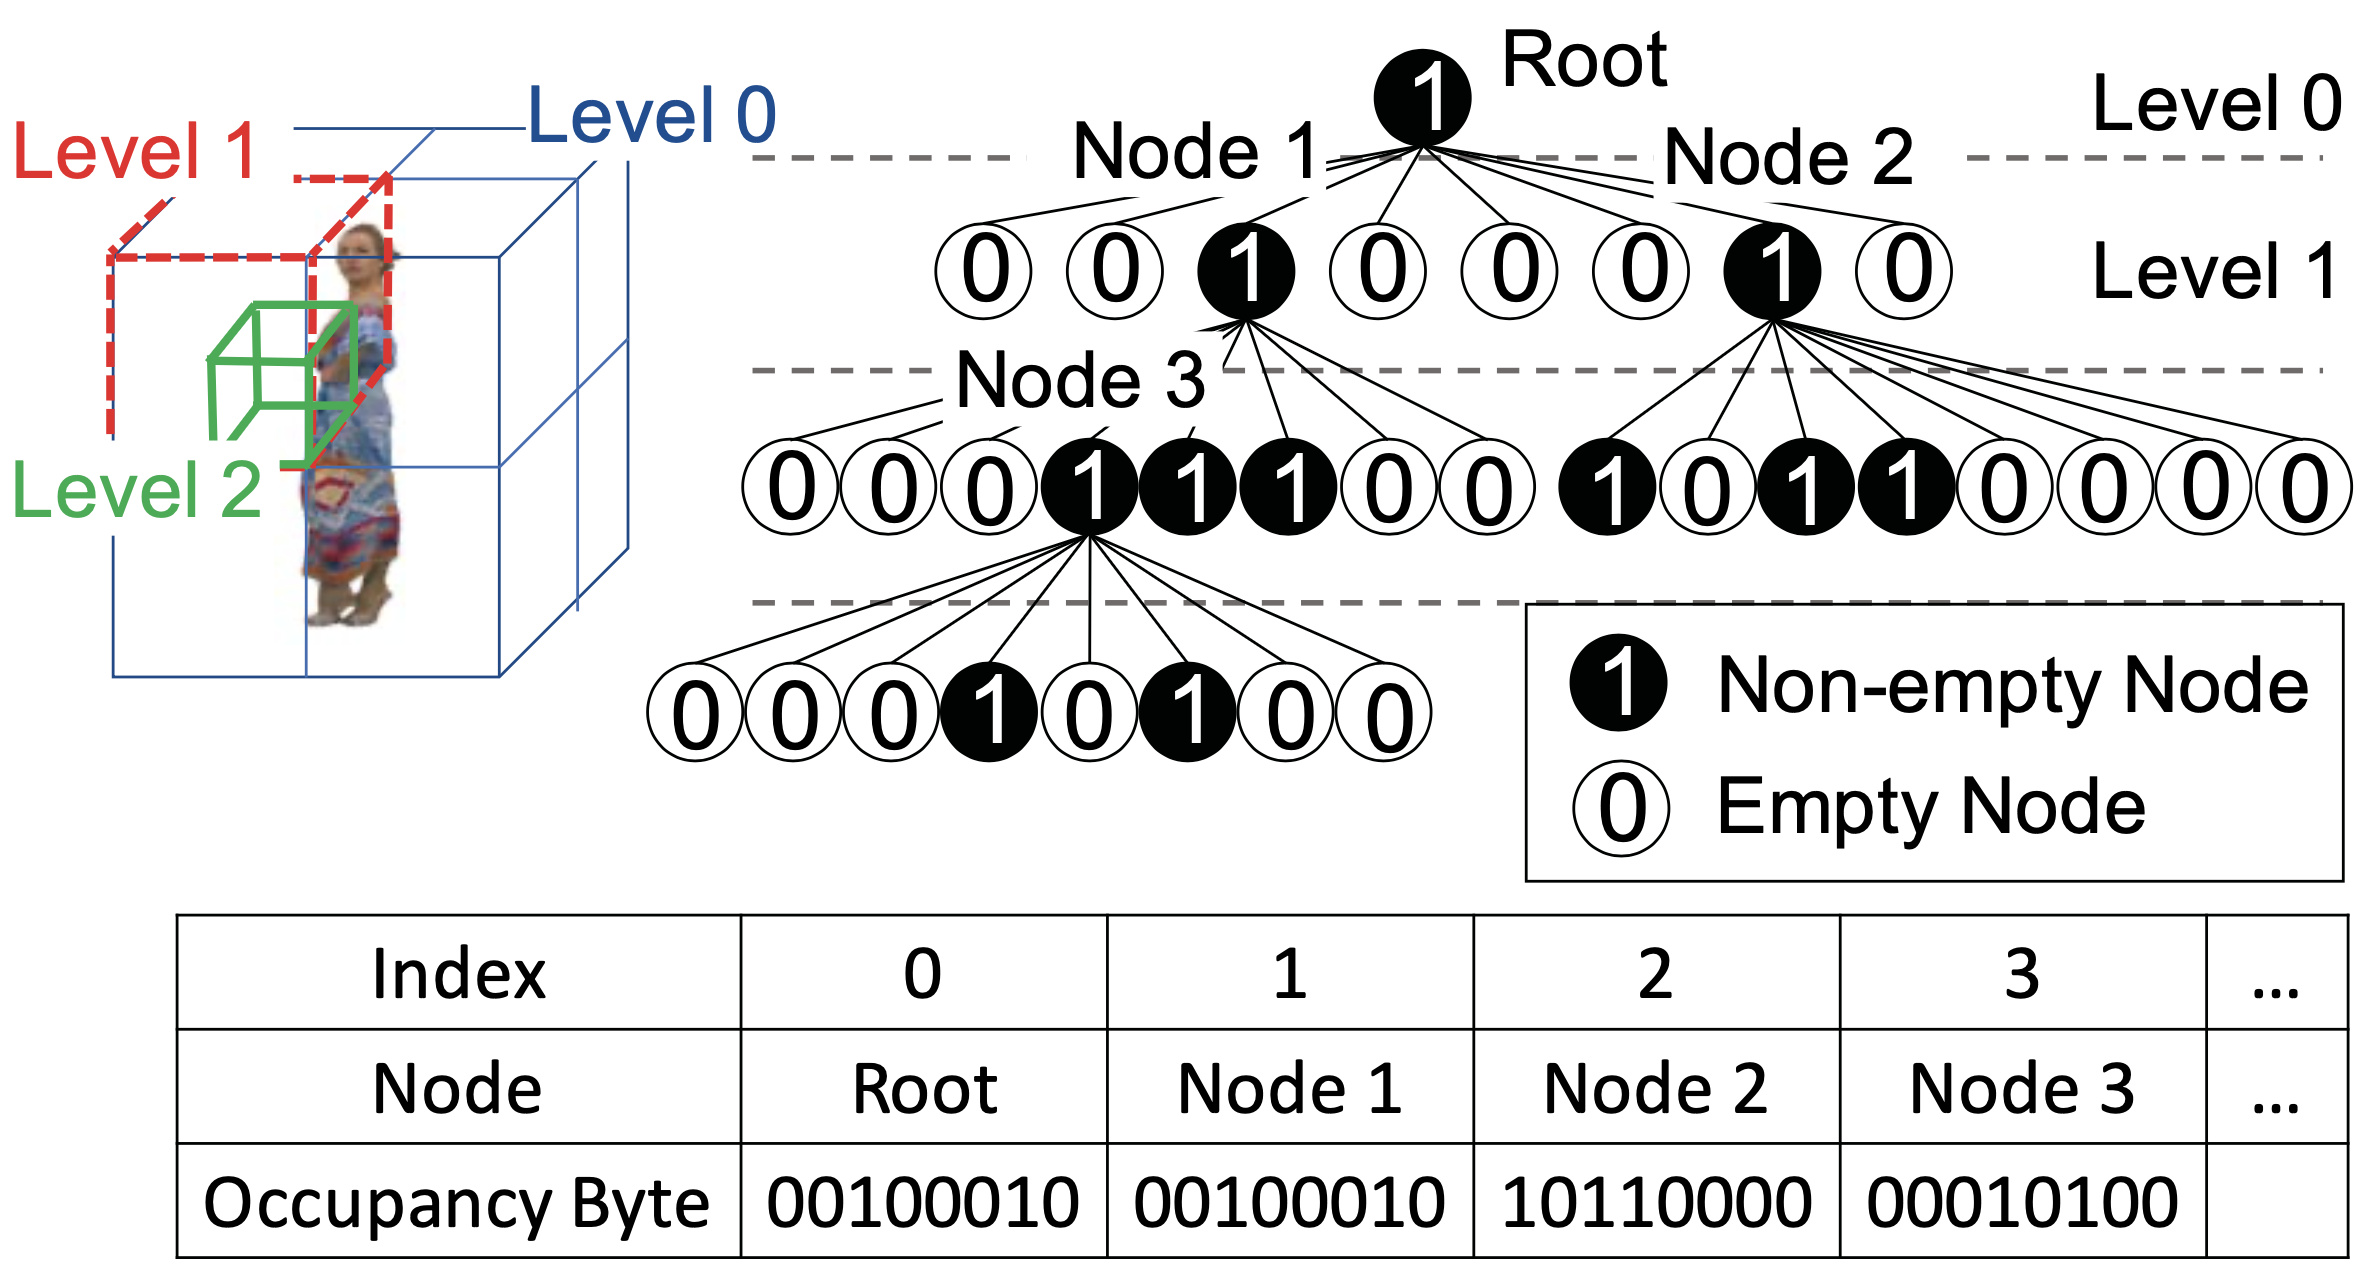
\includegraphics[width=\columnwidth]{figures/octree.png}
%   \caption{Octree. \raj{Taken from GROOT paper. Replace it with yours}}
%   \label{fig:octree}
% \end{figure}

\parab{The Octree Data Structure.}
\begin{figure}[t]
  \centering
  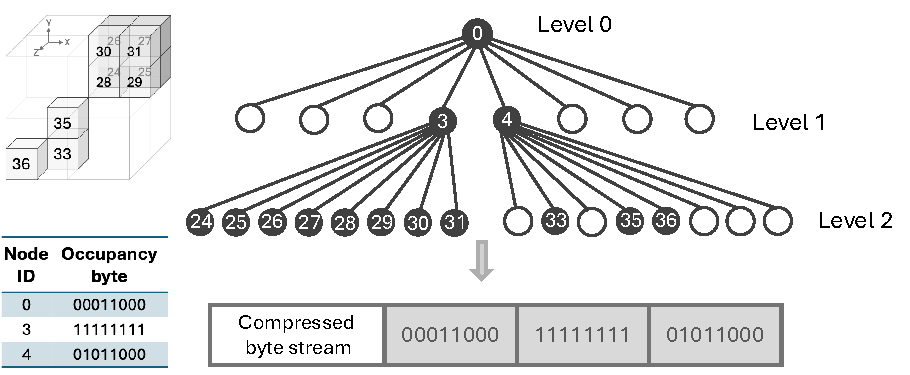
\includegraphics[width=\textwidth]{figures/octree.pdf}
  \caption{An example of an octree with some occupied voxels.}
\label{fig:octree}
\end{figure}
%
After voxelization, many voxels are often empty and only a small fraction of voxels are occupied by Gaussians.
%
An octree~\cite{octree-orig1982} efficiently encodes the positions of occupied voxels to exploit sparsity and spatial locality.
%
It recursively partitions the 3D space into octants (8 equally-sized child nodes), creating a tree structure where each node represents a cubic region of occupied space.

Consider the octree in~\cref{fig:octree}.
%
The root node represents the entire 3D space, and its 8 child nodes represent the 8 equally-sized children.
%
The child nodes that are occupied (\textit{i.e.}, contain at least one Gaussian) can be further subdivided into their own child nodes.
%
The process continues until we reach a leaf node that contains a single occupied voxel. 

This structure can efficiently encode occupancy.
%
Each internal tree node uses a byte, where each bit indicates whether the corresponding child node is occupied (1) or empty (0).
%
For example, if the fourth and fifth bits are set to 1, it means that the fourth and fifth child nodes are occupied, while the rest are empty (\cref{fig:octree}).

\parab{Recursive Octree Encoding.}
%
3-D compression must \textit{construct} the octree (\textit{i.e.}, determine octants and their occupancy), then \textit{encode} (\textit{i.e.}, serialize) the octree into a bitstream.
%
Both of these can be accomplished with a single sequential \textit{level-order} traversal from the root to the leaves; a reference implementation of G-PCC~\cite{gpcc-github} uses this approach.
%
This algorithm starts from the root, determines the occupancy of its child octants, then writes out the occupancy byte of the root.
%
It then recursively repeats the process for each child in a fixed sequence (\textit{i.e.}, if children are numbered $0..7$, it visits the children in that order), and stops when all occupied voxels form the leaves.

The output of this algorithm is a sequence of bytes representing occupancy at various nodes of the octree.
%
The total number of bytes in this sequence is proportional to the number of occupied voxels $\hat{N}_v$, which is often more compact than recording the occupancy of all $2^{3J}$ voxels.%\eduardo{I think the value of octree coding is not that its compressed size is proportional to $\hat{N}_v$, because even the naive approach of just sending the integer coordinates directly uses $3J \hat{N}_v$ bits. The advantage of the octree is that for surface like objects, it can reduce the $3J$ factor to a constant independent of the bit depth. In the original RAHT paper \cite{de2016compression} (Equation 5), they estimate that for smooth surfaces, octree encoding requires about $\frac{8}{3}$ bits per voxel. This is very close to actual estimates in point clouds, and close to our compressed 3DGS rates. }

In \cref{fig:octree}, for example, only two children of the root node (the 4th and the 5th) contain at least one occupied voxel, so its occupancy byte is $00011000$.
%
This forms the first byte of the output bitstream.
%
The second byte corresponds to the root's 4th child, all of whose children are occupied, so its occupancy byte is $11111111$, and so on.

%% The decoder can reconstruct the octree by reading the occupancy bytes level by level and determining which child nodes are occupied based on the bits set to 1.
%% %
%% To do this, it must know the value of $J$, which is usually passed as metadata along with the bitstream.
%% %
%% The decoder starts from the root node and reads the occupancy bytes level by level to determine which child nodes are occupied based on the bits set to 1.
%% %
%% At each level, the decoder finds the number of occupied nodes using the metadata and extracts the occupancy bytes for each node (parent). 
%% %
%% For each of these parent nodes, it adds a child to the octree for each bit set to 1 in the occupancy byte, and adds the child node to the list of nodes to be processed at the next level.
%% %
%% For example, in \cref{fig:octree}, the decoder would read the first byte, and determine that the 3rd and 7th children of the root are occupied.
%% %
%% It would then know that the next byte in the encoded bitstream corresponds to the 3rd child, and the one after that to the 7th, and so on.
%% %
%% This process continues until the decoder reaches the leaf nodes at depth $J$, which correspond to the occupied voxels.
%% %
%% The decoder obtains the reconstructed voxelized positions by calculating the center coordinates of the leaf node voxels.

%% %
%% Given our voxelized \gs model, we can construct such an octree by starting from the root node that represents the tight bounding box with dimension $2^J \times 2^J \times 2^J$.
%% %
%% The leaf nodes of the octree correspond to the occupied voxels in the voxelized \gs model.
%% %
%% Thus, $J$ is the depth of the octree, and the number of leaf nodes is equal to the number of occupied voxels $\hat{N}_v$.

%% Every node of an octree can be represented as a occupany byte, where each bit indicates whether the corresponding child node is occupied or empty.
%% %
%% The octree can be encoded into a bitstream by traversing the tree in level-order and writing the occupancy bytes of all nodes at each level contiguously.
%% %
%% Since, occupany bytes only encode nodes that are occupied, the total number of bytes required to encode the octree is proportional to the number of occupied voxels $\hat{N}_v$, which is much smaller than storing all $2^{3J}$ voxels.
%% %
%% This makes octree coding an efficient way to encode the positions of occupied voxels in a compact bitstream. The decoder can reconstruct the octree by reading the occupancy bytes level by level and determining which child nodes are occupied based on the bits set to 1.

\subsection{GPU-accelerated Octree Encoding}\label{sec:octree-encode-gpu}

\gsnfs{} parallelizes octree construction and encoding on the GPU.
%
Before describing this algorithm, we explain why this is a challenge, and how prior work has attempted to accelerate octree construction and encoding.
%
The next subsection describes GPU-accelerated octree decoding.

%% Traditionally, octree is used to hold $(x,y,z)$ positions of points in a point cloud. 
%% %
%% Octree based encoding consists of 2 steps: (a) octree construction and (b) bitstream generation.
%% %
%% Octree construction starts with voxelized positions (within tight bounding box around the point cloud) and builds a tree structure by recursively subdividing the 3D space into octants~\cite{octree-orig1982,gpcc}.
%% %
%% Due to sparse distribution of points, octree data structure efficiently holds only the occupied voxels, which is much smaller than all the voxels in the 3D space.
%% %
%% The depth of the octree $J$ is determined by the resolution of the voxel grid, and the leaf nodes correspond to the occupied voxels, which holds the voxelized positions.
%% %
%% The octree is then encoded into a bitstream to generate the final compressed representation of the geometry.
%% %
%% Each node of the octree represented by an occupancy byte, where each bit indicates if a child node (out of 8 children) is occupied, given by 1, or empty (given by 0).
%% %
%% A child is occupied if there is at least one point in its octant.
%% %
%% The occupancy bitstream is generated by traversing the octree in level-order and writing the occupancy bytes of all nodes at each level contiguously~\cite{octree-comp2002,octree-comp2006}.
%% %
%% The occupancy bitstream is further compressed using entropy coding techniques such as RLGR to generate the final compressed geometry bitstream~\cite{gpcc}.

%% Decoding the compressed bitstream to extract the voxelized positions first involves entropy decoding followed by reconstructing the octree structure from the occupancy bytes.
%% %
%% To help the decoder reconstruct the octree, the encoder needs to add metadata to the bitstream header such as the depth of the octree $J$, and the number of nodes at each level of the octree.
%% %
%% The decoder starts from the root node and reads the occupancy bytes level by level to determine which child nodes are occupied based on the bits set to 1.
%% %
%% At each level, the decoder finds the number of occupied nodes using the metadata and extracts the occupancy bytes for each node (parent). 
%% %
%% For each of these parent nodes, it adds a child to the octree for each bit set to 1 in the occupancy byte, and adds the child node to the list of nodes to be processed at the next level.
%% %
%% This process continues until the decoder reaches the leaf nodes at depth $J$, which correspond to the occupied voxels.
%% %
%% The reconstructed voxelized positions are then obtained by calculating the center coordinates of the leaf node voxels.

%% %
%% Today, 2D video codecs such as H.264 and H.265 are implemented on GPU, which allows for real-time encoding and decoding of high-resolution videos.
%% %
%% Since \gs data inherently resides in GPU memory during training and rendering, it is critical to implement the entire compression pipeline on GPU to avoid costly memory copy between CPU and GPU.
%% %
%% The first step in to develop a highly parallel octree encoding algorithm that can be efficiently implemented on GPU.

\begin{table}[t]
  \centering
  {%\scriptsize
  \begin{tabular}{lp{0.7\textwidth}}
    \hline
    \textbf{Works} & \textbf{Quote}  \\ \hline
    Zhou~\cite{octree-gpu2011} & ``Creating an octree for point clouds directly on the GPU, however, is very difficult, mainly because of memory allocation and pointer creation.'' \\ \hline
    GROOT~\cite{groot} & ``While the tree structure efficiently handles the sparsity of 3D data and subdivides only the volumes where the point exists, the irregularity requires traversing the serialized byte stream and recursively calculating the child node geometry. The exact positions that represent intermediate nodes depend on the occupancy of their ancestors, which cannot be parallelized.'' \\ \hline
  \end{tabular}}
  \caption{Parallelization challenges for octree encoding reported in prior work.}
  \label{tab:octree-challenge}
\end{table}

\parab{Challenges.}
%
Recursive octree construction is inherently sequential.
%
State-of-the-art point cloud compression algorithms~\cite{gpcc,draco,pcl} implement sequential CPU-based octree construction and encoding.
%
Constructing the octree requires traversing the tree top-down and creating nodes and pointers.
%
This is difficult to efficiently parallelize on a GPU since the memory layout of the tree can be irregular, and tree-traversal might require pointer-chasing, resulting in GPU thread stalls while waiting for memory accesses to complete~\cite{octree-gpu2011,octree-cpu2020,groot}.
%
Generating the occupancy bitstream also requires a tree traversal in level-order and pointer-chasing to determine the occupancy byte of a node depending on existing children, which can be inefficient on a GPU.
%
\cref{tab:octree-challenge} includes quotes from prior work~\cite{octree-gpu2011,groot} that illustrate the difficult of parallelizing octree encoding.

\parab{Prior Work on Parallelization.}
%
One line of work has explored CPU parallelism for octree construction and encoding.
%
ViVo~\cite{vivo}, MeshReduce~\cite{meshreduce}, and MetaStream~\cite{metastream} use coarse-grained CPU parallelism by partitioning the 3D points into separate blocks, generating the octree encoding independently for each block and concatenating these encodings.
%
Others~\cite{octree-cpu2020,groot} employ slightly more sophisticated hybrid CPU-GPU strategies.
%
For example, Groot~\cite{groot} sequentially constructs the octree top-down up to a certain depth $d$, then generates encodings in parallel for each occupied voxel (on a GPU) by traversing the tree bottom-up up to level $d$.

Another line of work~\cite{octree-cpu2008,octree-gpu2011,octree-gpu2012} has achieved GPU-accelerated parallelization of octree construction.
%
They linearize the positions in 3D to a 1D list using a space-filling curve (the Morton code, described below) while preserving spatial locality~\cite{morton-code-spc}.
%
Thus, the generated octree is not explicitly represented as a tree structure, but rather as arrays of indices in the space-filling curve for each node at a certain level. 
%
In these approaches, however, \textit{encoding is still sequential}, since that requires an in-order tree traversal.
%
\gsnfs{} uses a similar space-filling curve, but parallelizes both construction and encoding on a GPU.

%% Prior works~\cite{octree-cpu2008,octree-gpu2011,octree-gpu2012} have attempted to parallelize the octree construction by constructing the tree from leaf to root.
%% %
%% The key idea is to linearlize the positions in 3D to a 1D list using morton codes, which is a space-filling curve that maps 3D coordinates to a single dimension while preserving spatial locality~\cite{morton-code-spc}.
%% %
%% morton codes allow for $O(1)$ parent-child determination, which enables parallel construction of the octree without explicit nodes and pointers.
%% %
%% The generated octree is not explicitly represented as a tree structure, but rather as arrays of morton indices for each node at a certain level. 
%% %
%% These works used this representation for fast neighbor selection~\cite{octree-gpu2012} and surface reconstruction~\cite{octree-gpu2011}, but they did not generate the occupancy bitstream which is required for octree-based compression.
%% This still need to be generate in CPU~\cite{gpcc,draco}.
%

% \begin{figure}[t]
%   \centering
%   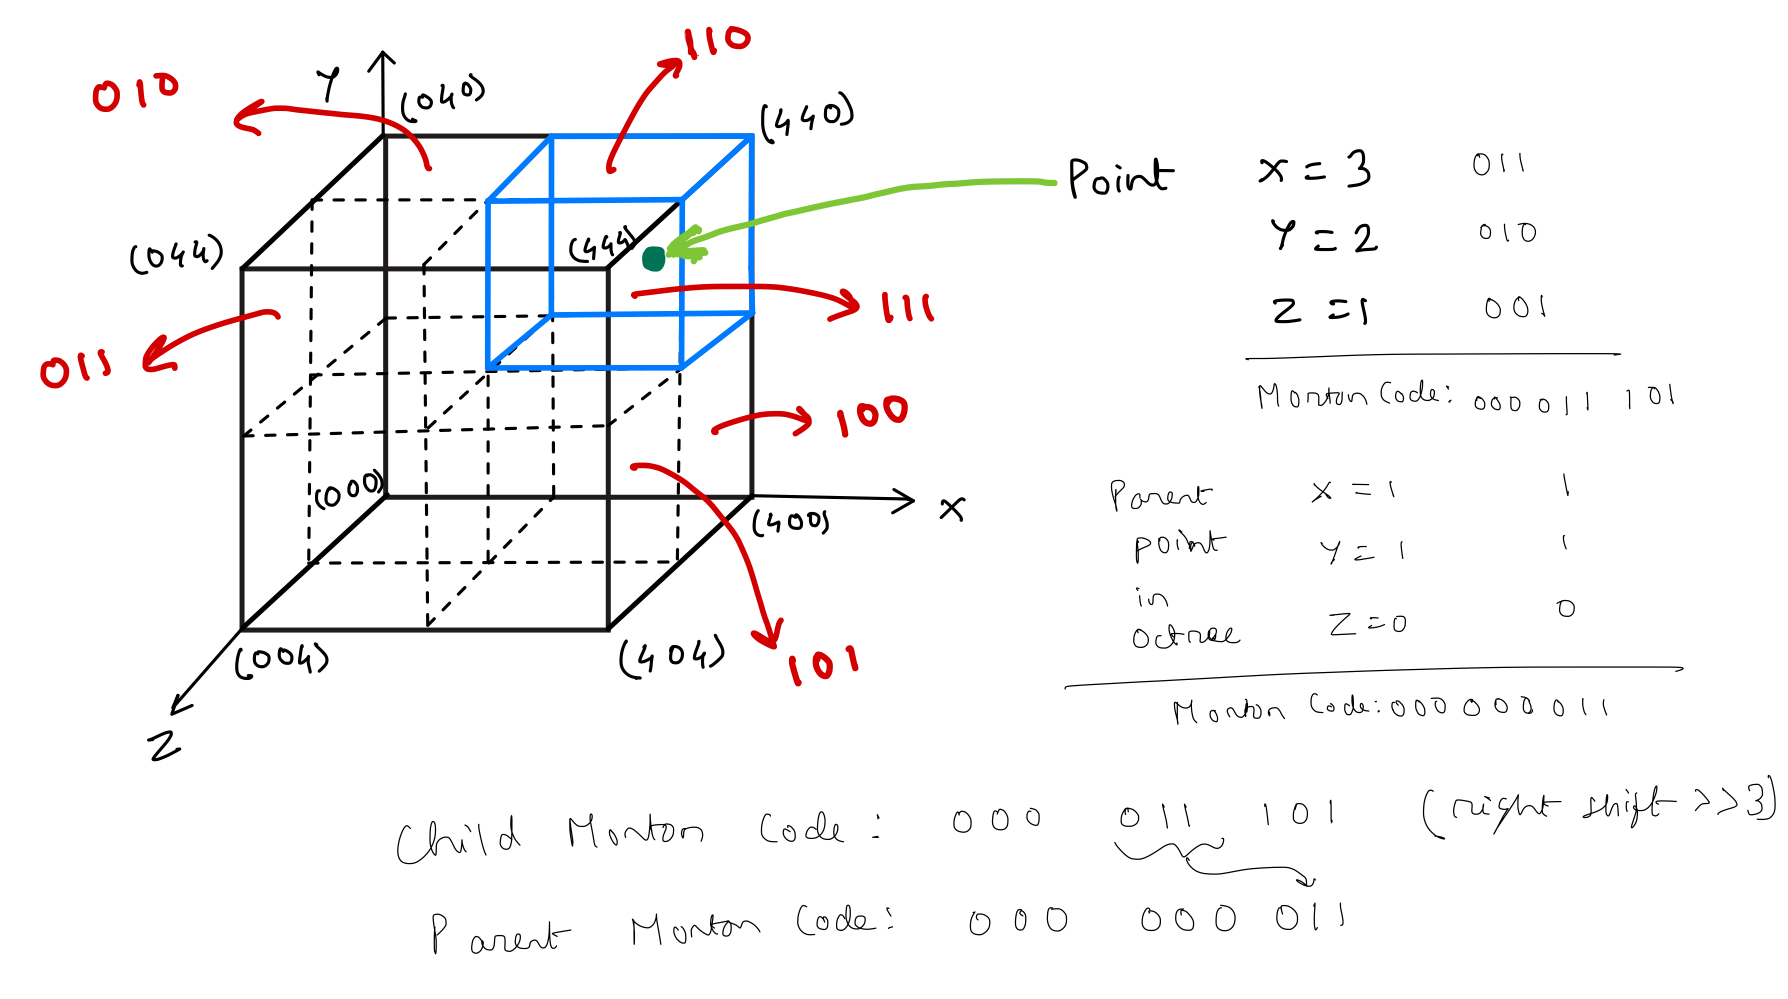
\includegraphics[width=\columnwidth]{figures/morton.jpeg}
%   \caption{Undestanding morton codes. \raj{Replace it with your drawio figure}}
% \label{fig:morton}
% \end{figure}

\begin{figure}[t]
  \centering
  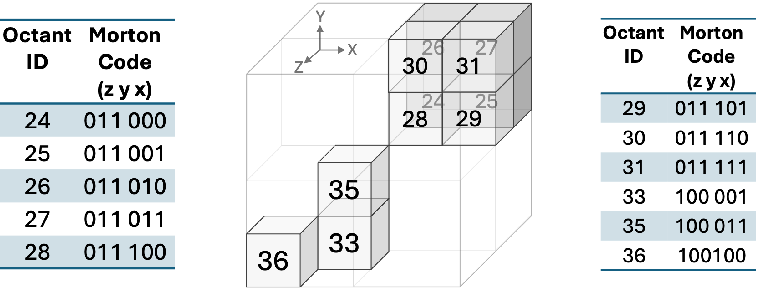
\includegraphics[width=\textwidth]{figures/morton_codes_octant.pdf}
  \caption{This figure shows the Morton codes of the occupied voxels in \cref{fig:octree}.}
\label{fig:morton}
\end{figure}

\parab{Morton Codes.}
%
The key to our GPU-accelerated octree encoder is to never build explicit tree pointers.
%
Rather, we represent each occupied voxel by its \emph{Morton code}~\cite{morton-code-spc}, which is a bit-interleaving of its integer voxel coordinates.
%
For a voxelized coordinate $\hat{v}=(x,y,z)\in\{0,\ldots,2^J-1\}^3$, the Morton code is a bit string $z_{J-1}y_{J-1}x_{J-1}\ldots z_0y_0x_0$ where $x_b,y_b,z_b$ are the $b$-th least-significant bits of $x,y,z$.

For example, consider the voxelization shown in~\cref{fig:morton}, which depicts a $4\times4\times4$ voxel grid ($J=2$) with 11 occupied voxels.
%
The occupied voxel with ID $33$ has coordinates $(1,0,2)$ so its Morton code is $100001$.
%
The Morton code is obtained by first taking the most significant bits of the 3 coordinates ($100$) in the order from $z-x$, followed by the next most significant bits (0 for the z-coordinate value of 2, 0 for the y-coordinate value of 0, and 1 for the x-coordinate value of 1), and so on.

The Morton code has three properties crucial for GPU-acceleration of octree construction, encoding, and decoding.
%
First, it preserves spatial locality: when we sort the voxels by their Morton code, voxels near each other in space will be near each other in the sorted order~\cite{morton-code-spc}.
%
For example, if in~\cref{fig:morton}, the voxel with ID $33$ and coordinate $(1,1,2)$ is also occupied, it would have the Morton code $100011$.
%
This differs from the Morton code of its neighboring voxel $(1,0,2)$ only in the last 3 digits.
%
This property ensures memory locality if voxels are laid out in GPU memory in Morton order, and avoids non-local memory access overheads.

Second, the Morton code for the parent of a voxel is a prefix of the voxel's Morton code.
%
In \cref{fig:morton}, the parent of $(1,0,2)$ (ID $33$) has the code $100$, which can be obtained by shifting the voxel's Morton code three bits to the right.
%
Conversely, to obtain the Morton code of, say, the 5th child of an octree node, we simply append $101$ to the node's Morton code.

Third, given the Morton code for a voxel, we can obtain its voxelized coordinates using the definition of the Morton code.
%
In our example, given the code $100011$, the first coordinate is obtained by concatenating every third bit starting from position 3, the second coordinate by doing so from position 2, and so on, resulting in the coordinate $(1,1,2)$.

%% (b) make octree topology \emph{implicit}: if $c_m$ is morton code for child node, its parent's code $p_m$ is simply $p_m = c_m \gg 3$, \ie dropping the last three interleaved bits; conversely, if $p_m$ is a parent code, its eight candidate children have morton codes $[(p_m \ll 3) \;|\; i]_{i=0}^7$, where $i$ is the child index.
%% %
%% Consider the example in \cref{fig:morton}, where we have a $4\times4\times4$ voxel grid ($J=2$) with one occupied voxel.
%% %
%% Let's consider the morton code for the root node, which the bounding box of the entire grid, is 0. 
%% %
%% The bounding box gets subdivided into 8 child octants, thus the child morton codes $[000,001,\ldots,111]$ uniquely identify each child.
%% %
%% If one of the child octants is occupied, say the one with morton code 5, then its parent code is simply $5 \gg 3 = 0$ (root node), which is the root node.
%% %
%% If the octant with morton code 5 is further subdivided, its children have morton codes $[40,41,\ldots,47]$, which can be computed by left-shifting the parent code and adding the child index, \ie $5 \ll 3 = 40$ is the first child, and $5 \ll 3 + 7 = 47$ is the last child.
%% %
%% Conversely, the parent code of any of these children is simply $[40,41,\ldots,47] \gg 3 = 5$.
%% %

Thus, if given the Morton code for an occupied voxel, it is an $O(1)$ operation to determine its parent.
%
Conversely, if all octree nodes are sorted in Morton order, then a parent can in an $O(1)$ operation determine its child's Morton code, and look up its occupancy status.
%
Finally, in $O(1)$, given a node's Morton code, we can obtain its voxel coordinates.

Before explaining how we use these properties to construct, encode and decode octrees, we describe how we parallelize voxelization (\cref{sec:background}).
%
This is important since voxelization precedes octree construction.
%
We require all steps in \gsnfs{} to be GPU-resident to avoid data movement costs (\cref{sec:appr-chall-contr}).

\parab{Voxelization.}
%
Voxelization (a) discretizes Gaussian positions and (b) merges Gaussian attributes (by averaging them) of Gaussians at the same discretized positions.
%
The input to this step is an $N \times C$ tensor for a \gs{} frame with $N$ Gaussians, with each Gaussian having $C$ attributes.
%
Step (a) is simple to parallelize on a GPU by launching one thread per Gaussian, which computes the voxel coordinates (\cref{sec:background}) of the Gaussian.
%
This step also computes the voxel's Morton code, and creates an array sorted by the Morton code that contains a pointer to the Gaussian.
%
We use a 64-bit Morton code to support octree depths up to $J=21$, which is sufficient for all scenes of interest~\cite{mesongs}.
%
If $J\leq 21$, we set to zero the unused most-significant bits in the Morton code.

In this array, Gaussians belonging to the same voxel are contiguous; we identify these \textit{clusters} using standard PyTorch operations.
%
Then, we launch one GPU thread for each cluster to average the attributes of Gaussians in that cluster.
%
The output of this process is an $N_v \times C$ tensor, where $N_v$ is the number of occupied voxels.
%
This is sorted by Morton order, and forms the input to the next step.

\parab{Octree construction.}
%
In contrast to the recursive top-down approach (\cref{sec:background}),
our construction identifies, \textit{bottom-up}, occupied parents of occupied voxels, and occupied internal nodes up the octree (\cref{fig:octree}).
%
Let $L_J$ be an array of occupied voxels, sorted by Morton order, obtained directly from the input tensor.
%
We launch one GPU thread per occupied voxel; this thread computes the parent's Morton code and writes this to a new list $L_{J-1}$.
%
This array contains parents of occupied voxels in Morton order, but can have duplicates, since multiple occupied voxels can have the same Morton code.
%
We use CUDA's \texttt{unique} primitive to compact duplicates in parallel, so $L_{J-1}$ has exactly one instance of an occupied parent.

We can now repeat this process to find the next-level occupied parents (\textit{i.e.}, parents of occupied parents) up to the root level.
%
The output of this process is a list of Morton codes for the occupied nodes at each level, \ie $L_0,\ldots,L_J$, where $L_0$ has the root node, $L_J$ has the leaf nodes, and $L_d$ has the occupied nodes at depth $d$.
%% At depth $J-1$, the parents of the leaf nodes need to be identified.
%% %
%% Recall that shifting a morton code right by 3 bits gives the parent code.
%% %
%% Each thread can independently compute the parent code $p_m$ from the morton code of a leaf node $c_m$ by right-shifting its morton code by 3 bits, $p_m = c_m \gg 3$.
%% %
%% Since the morton code is sorted and bit right-shift preserves the order, the parent morton codes are also sorted but not unique.
%% %
%% Unlike other GPU octree construction tecnhniques~\cite{octree-cpu2008,octree-gpu2011,octree-gpu2012}, we only sort the leaf nodes, and we never sort the internal nodes.
%% %
%% But, multiple leaf nodes can have the same parent code, so we need to compact duplicates to get the unique parent codes.
%% %
%% We use CUDA's unique primitive to compact duplicates in parallel, which gives us the list of occupied parent nodes at depth $J-1$.
%% %
%% Similar to leaf level, we arrive at a list of unique sorted morton codes for the occupied nodes at depth $J-1$.
%% %
%% We repeat this process iteratively until we reach the root node at depth 0, which has a single code 0 for the root node.

\parab{Bitstream generation.}
%
From these lists, the encoder must emit the octree occupancy bitstream.
%
Each internal node contributes exactly one occupancy byte, whose $i$-th bit is set if child $i$ exists.
%
This step requires us to compute the occupancy byte for each internal node.
%
To compute this, a node must: (a) determine the Morton codes of its children and (b) identify which children are occupied.

Given a parent code $p_m\in L_d$, the Morton prefix of its children can be obtained by $c_m = p_m \ll 3$.
%
The eight possible children are therefore the contiguous code range $[c_m,c_m+7]$.
%
To compute the occupancy byte for $p_m$, we need to check which of these eight candidate child codes exist in the child list $L_{d+1}$.
%
This requires searching for the child codes in $L_{d+1}$.

We make 2 observations that make this search efficient. 
%
First, all children with Morton codes in the range $[c_m,c_m+7]$ must appear contiguously in the sorted list $L_{d+1}$.
%
Second, we can perform a binary search for the first occupied child code $\geq c_m$ in $L_{d+1}$, since that listed is sorted.

To compute the occupancy bytes for all octree nodes, we use a \textit{top-down} approach.
%
We compute occupancy bytes for nodes in $L_d$ before doing so for nodes in $L_{d+1}$.
%
At level $L_d$, our octree encoder launches a custom CUDA kernel\footnote{For efficiency, when necessary, we replace PyTorch operations with custom CUDA kernels to improve encoding speed.}
with one thread per parent node $p_m$ in $L_d$.
%
It initializes $p_m$'s occupancy byte to 0.
%
Then, the thread for $p_m$ performs the following steps:.
(i) compute $c_m = p_m \ll 3$;
(ii) binary-search $L_{d+1}$ to find the first occupied child code $\geq c_m$;
(iii) scan forward over at most 8 entries until the child code exceeds $c_m+7$;
(iv) set bit for every child code $c_m$ found.
%
The thread then writes its occupancy byte to a known location in the GPU buffer.

% \ramesh{Add a figure that uses the running example from \cref{fig:octree} and \cref{fig:morton} to show how, for the top-level, the above steps work.}

% \ao{Since we already have a block diagram, refer to it here so that it's easier to understand the various blocks in the system.}
At the end, all the occupancy bytes are written in order, similar to \cref{fig:octree}.
%
To improve compression efficiency, \gsnfs{} then runs a GPU-based entropy encoder (\cref{fig:architecture_gsnfs}), ANS~\cite{nvidia_nvcomp}.

\parab{Detailed Algorithm.} 
%
\begin{algorithm}[t!]
  \caption{GPU Octree{}'s Encoding from Voxelized Positions}
  \label{algo:octree-encode-gpu}
\SetAlgoLined
\DontPrintSemicolon

\SetKwInOut{Input}{Input}
\SetKwInOut{Output}{Output}

\SetKwFunction{Morton}{Morton}
\SetKwFunction{RadixSort}{RadixSort}
\SetKwFunction{Unique}{Unique}
\SetKwFunction{Parent}{Parent}
\SetKwFunction{OccKernel}{OccKernel}
\SetKwFunction{Concat}{Concat}
\SetKwFunction{Append}{Append}
\SetKwFunction{BinarySearch}{BinarySearch}

\Input{Voxelized integer positions $\hat{V}=\{(\hat{x}_i,\hat{y}_i,\hat{z}_i)\}_{i=1}^{\hat{N}_v}$ on GPU; octree depth $J$}
\Output{Serialized octree bitstream $B_{occ}$}

\BlankLine
\tcp*[l]{Step 1: Morton codes for leaf voxels}
\ForPar{$i \gets 1$ \KwTo $\hat{N}_v$}{
  $m_i \gets \Morton(\hat{x}_i,\hat{y}_i,\hat{z}_i, J)$
}
$L_J \gets \Unique(\RadixSort(\{m_i\}))$ \tcp*{leaf nodes}

\BlankLine
\tcp*[l]{Step 2: Level-synchronous octree construction}
\For(\tcp*[f]{bottom-up parents}){$d \gets J-1$ \KwTo $0$}{
  $L_d \gets \Unique(\{\, \Parent(c_m)\;|\;c_m\in L_{d+1}\,\})$ \tcp*{$\Parent(c_m)=c_m\gg 3$}
}

\BlankLine
\tcp*[l]{Step 3: Bitstream header}
$num\_levels \gets J+1$\;
$level\_sizes \gets (|L_0|,\ldots,|L_J|)$\;
$B_{occ} \gets \Append(B_{occ}, num\_levels, level\_sizes)$\;

\BlankLine
\tcp*[l]{Step 4: Breadth-first occupancy bitstream.}
\ForPar{$d \gets 0$ \KwTo $J-1$}{
  $B_d \gets \OccKernel(L_d, L_{d+1})$
  $B_{occ} \gets \Append(B_{occ}, B_d)$ \tcp*{contiguous bytes for level $d$}
}

\Return $B_{occ}$\;

\BlankLine
\textbf{Kernel \OccKernel($L_d,L_{d+1}$):}\;
\ForPar{$p \in L_d$}{
  $c_m^b \gets p \ll 3$ \tcp*{base child code}
  $occ \gets 0$ \tcp*{occupancy byte}
  $c_m \gets \BinarySearch(L_{d+1}, c_m^b)$
  \For{$k \gets 0$ \KwTo $7$}{
      \If{$L_{d+1}[c_m+k] \leq c_m^b+7$}{
        $occ \gets occ \;|\; \big(1 \ll (L_{d+1}[c_m+k]-c_m^b)\big)$\;
      }
      
  }
  Write $occ$ into $B_d$ at parent's index\;
}
\end{algorithm}
%
\cref{algo:octree-encode-gpu} summarizes our GPU octree encoder. 
%
Starting from voxelized integer coordinates, we first compute Morton codes for all occupied leaf voxels, then radix-sort and deduplicate them to obtain the leaf set $L_J$. 
%
The upper octree levels are constructed bottom-up by repeatedly mapping child codes to their parents and removing duplicates, yielding level-wise node sets $\{L_d\}_{d=0}^J$.

After the hierarchy is built, we serialize a compact occupancy bitstream. 
%
The header stores the number of levels and the node count of each level. 
%
The payload is then generated in breadth-first order: for each parent in level $L_d$, we produce one occupancy byte indicating which of its eight children are present in $L_{d+1}$. 
%
As shown in \cref{algo:octree-encode-gpu}, this is done by locating the base child Morton code and setting the corresponding bits for all valid children in the next level.

This construction avoids explicit pointer-based octree data structures and operates directly on sorted Morton codes, which is well suited to parallel primitives such as radix sort, deduplication, and batched searches. 
%
The resulting bitstream is a level-synchronous octree representation that can be decoded with the same breadth-first traversal order.

%% \parab{Parallelization template.}
%% Our parallelization strategy for octree construction is a simple level-synchronous approach. 
%% %
%% At each level, we launch one thread per node to perform a computation, then we gather the results in a list. 
%% %
%% This list is used to launch the next level of threads, and we repeat this until we reach the root node. 
%% %
%% We will use such level-synchronous heirarchy template for most of \gsnfs's algorithms, including RAHT, which we will describe later.

\subsection{GPU-Accelerated Octree Decoding}\label{sec:octree-decode-gpu}

\parab{Inputs and Output.}
%
The input to this algorithm is a sequence of occupancy bytes in the octree.
%
We obtain this from the output of the ANS entropy decoder.
%
The output of the algorithm is a list of voxelized positions of occupied voxels.
%
Each such position corresponds to a Gaussian, whose attributes we obtain as described in \cref{sec:gpu-raht}.

This algorithm also needs to know $J$, the depth at which the \gs{} frame was encoded, and the number of occupied nodes $n_d$ at each level $d$ in the tree.
%
Such information is encoded in the bitstream as \textit{metadata}. 
% by many encoders, not just \gsnfs{}.

% \parab{A Strawman Approach.}
% %
% Given the encoded bitstream obtained from the above octree encoding process, the decoder needs to extract the voxelized positions.
% %
% To do this, the decoder can process the occupancy bytes from the bitstream sequentially, starting with the first byte for the root's occupancy.
% %
% That byte determines which children are occupied; if $k$ children are occupied then the next $k$ bytes in the bitstream contain occupancy bits for those children.
% %
% From the first byte, we can also determine the voxel coordinates of the children.
% %
% The strawman approach can continue to recurse at each child, processing each child sequentially, until we reach depth $J$.

% A naïve parallelization of our strawman would launch one thread per octree node at each level of the tree to determine the occupied child nodes and build the octree bottom-up.
% %
% However, this requires the Morton codes for the occupied child nodes at each level to be included in the metadata.
% %
% Each Morton code requires 64-bits per occupied node, which is much larger than the 1 byte per node required by the occupancy bitstream, so this approach is clearly infeasible.
\parab{Prior work.}
%
GROOT and~\cite{octree-cpu2020} try to decode lower levels of the octree in parallel on a CPU, but most tree levels are still decoded sequentially on the CPU top-down.
%
We know of no other work that has GPU-accelerated decoding.

\parab{Octree decoding.}
%
Our octree decoding algorithm relies on properties of the Morton code.
%
We note that the first byte is the occupancy byte of the root.
%
From this, we can determine (a) which children are occupied, and (b) the Morton code of the children (both $O(1)$ operations).
%
We can repeat this process to obtain the Morton codes of all nodes in the tree, and eventually, the Morton codes of all occupied voxels.
%
From these, we can obtain the voxelized positions of the occupied voxels using the definition of the Morton code.

To parallelize this, we use a top-down level-synchronous approach (similar to the encoder), where, at each level $d$, we launch one thread per octree internal node.
%
For level $d$, we can determine from the metadata where the occupancy bytes for that level start and end.
%
But each node at that level can have a variable number of occupied children.
%
To determine the offset of the $k$-th occupied node, we first create an array per internal node that counts the number of occupied children (using the population count CUDA primitive), then do a CUDA prefix sum on that array to find the offset of this node's children in the occupancy bytes at level $d+1$.

The $k$-th occupied node writes the Morton codes of its occupied children into a separate array starting at the corresponding offset.
%
Then, the decoder launches one thread for each occupied thread at level $d+1$, and the process repeats.
%
After processing all levels, the decoder's output is a list of Morton codes for the leaf nodes, which correspond to the occupied voxels.
%
The decoder launches a final CUDA kernel to decode the Morton codes back into integer voxel coordinates by reversing the bit interleaving.

\parab{Detailed Algorithm.}
%
\begin{algorithm}[t!]
  \caption{GPU Octree Decoding}
  \label{algo:octree-decode-gpu}
\SetAlgoLined
\DontPrintSemicolon

\SetKwInOut{Input}{Input}
\SetKwInOut{Output}{Output}

\SetKwFunction{ReadHeader}{ReadHeader}
\SetKwFunction{ReadOcc}{ReadOccBytes}
\SetKwFunction{Popcount}{Popcount}
\SetKwFunction{ExScan}{ExclusiveScan}
\SetKwFunction{ExpandKernel}{ExpandChildrenKernel}
\SetKwFunction{ReconKernel}{ReconstructPointsKernel}
\SetKwFunction{MortonDec}{MortonDecode}
\SetKwFunction{Interleave}{InterleaveXYZ}

\Input{Compressed octree buffer $B$ on GPU; octree depth $J$}
\Output{Voxelized positions $\hat{V}$ on GPU; leaf Morton codes $L_J$ on GPU}
\BlankLine
\tcp*[l]{Step 1: Parse header.}
$(num\_levels,\ level\_sizes,\ ptr) \gets \ReadHeader(B)$\;

\BlankLine
\tcp*[l]{Step 2: Initialize root list (implicit root Morton code).}
$L_0 \gets [\,0\,]$

\BlankLine
\tcp*[l]{Step 3: Level-synchronous decoding.}
\For(\tcp*[f]{top-down levels}){$d \gets 0$ \KwTo $J-1$}{
  $M_d \gets |L_d|$\;
  $Occ_d \gets \ReadOcc(ptr, M_d)$ \tcp*{read $M_d$ bytes from $B$ into a GPU array}
  $ptr \gets ptr + M_d$\;

  \BlankLine
  \tcp*[l]{Count children per parent.}
  \ForPar{$p \gets 1$ \KwTo $M_d$}{
    $cnt[p] \gets \Popcount(Occ_d[p])$\;
  }

  \BlankLine
  \tcp*[l]{Find total children at $d+1$.}
  $off \gets \ExScan(cnt)$
  $T \gets off[M_d] + cnt[M_d]$\;
  Allocate $L_{d+1}$ of length $T$\;

  \BlankLine
  \tcp*[l]{Expand children.}
  \ExpandKernel$(L_d, Occ_d, off, L_{d+1})$ with $M_d$ threads\;
}

\BlankLine
\tcp*[l]{Step 6: Get voxel coordinates at leaf.}
$\hat{N}_v \gets |L_J|$\;
$shift \gets J_v - J$\;
Allocate $\hat{x}[1{:}\hat{N}_v],\hat{y}[1{:}\hat{N}_v],\hat{z}[1{:}\hat{N}_v]$\;
Launch \ReconKernel$(L_J, shift, \hat{x},\hat{y},\hat{z})$ with $\hat{N}_v$ threads\;
$\hat{V} \gets \Interleave(\hat{x},\hat{y},\hat{z})$ \tcp*{Reverse Morton Code.}

\Return $(\hat{V}, L_J)$\;
\end{algorithm}

\begin{algorithm}[t!]
  \caption{\texttt{expand\_children\_kernel}: Expand occupied children and generate Morton codes}
  \label{algo:octree-expand-children-kernel}
\SetAlgoLined
\DontPrintSemicolon
\SetKwInOut{Input}{Input}
\SetKwInOut{Output}{Output}

\Input{Parent Morton codes $L_d[1{:}M_d]$; occupancy bytes $Occ_d[1{:}M_d]$; write offsets $off[1{:}M_d]$}
\Output{Child Morton codes $L_{d+1}[1{:}T]$}

\ForPar{$p \gets 1$ \KwTo $M_d$}{
  $parent \gets L_d[p]$\;
  $occ \gets Occ_d[p]$\;
  $base \gets parent \ll 3$ \tcp*{base child Morton code}
  $w \gets off[p]$ \tcp*{exclusive-scan start offset for this parent}
  \For{$i \gets 0$ \KwTo $7$}{
    \If{$occ \wedge (1 \ll i)$}{
      $L_{d+1}[w] \gets base + i$\;
      $w \gets w + 1$\;
    }
  }
}
\end{algorithm}
%
\cref{algo:octree-decode-gpu} summarizes our GPU octree decoder.
%
The GPU decoder reconstructs voxelized geometry by replaying the serialized occupancy stream in a level-synchronous manner, without building any explicit tree pointers.
%
Starting from the implicit root Morton code ($L_0=\{0\}$), for each depth $d$ it reads the $|L_d|$ occupancy bytes, counts the number of occupied children per parent (population count), and performs an exclusive prefix-sum to compute disjoint write offsets for the next-level array.
%
It then launches \texttt{expand\_children\_kernel} (Alg.~\ref{algo:octree-expand-children-kernel}), which generates each occupied child Morton code in $O(1)$ via $(parent \ll 3)+i$ and writes all children contiguously into $L_{d+1}$, avoiding atomics despite variable fan-out.
%
Repeating this from $d=0$ to $J{-}1$ yields the leaf Morton codes $L_J$, which are finally decoded into integer voxel coordinates (and optionally interleaved) in a parallel post-pass.
%
Overall, decoding preserves the same breadth-first structure as the encoder while turning the key sequential dependency (unknown next-level size) into a standard GPU pattern: count $\rightarrow$ prefix-sum $\rightarrow$ parallel scatter.

% \ramesh{Add a small example, consistent with the encoding example.}

%% \gsnfs uses the same level-synchronous approach as the encoder, where we launch one thread per parent node at each level to determine the occupied child nodes and generate their morton codes.
%% %
%% But, each parent has a variable number of occupied children, ranging from 0 to 8 depending on sparsity.
%% %
%% Therefore, the morton code list for the next level $L_{d+1}$ is a variable-length concatenation of each parent's children.
%% %
%% On the GPU, variable output sizes require computing write offsets so that each parent thread writes its children into a disjoint region of the output array without atomics.
%% %
%% We compute these offsets via a prefix sum over the per-parent child counts.
%% %
%% Each element of the prefix sum provides the indices to the children's list, where the parent thread writes the morton codes of its occupied children.

%% The decoder extracts the octree depth from the first 4 bytes of the bitstream header and the number of nodes at each level from the next $4J$ bytes of the header.
%% %
%% At each level, the decoder reads the occupancy bytes for all nodes at that level from GPU memory.
%% %
%% Then, it launches a CUDA kernel that counts the number of occupied children for each parent node by counting the number of set bits (using population count CUDA primitive) in the occupancy byte.
%% %
%% From the child counts, we compute the write offsets for each parent node by performing a parallel prefix sum.
%% %
%% Again, it launches a CUDA kernel with one thread per node to generate the morton codes for its occupied children.
%% %
%% It writes the codes at the offsets calculated by the prefix sum.
%% %

%\raj{Add complexity analysis of octree encoding and decoding.}
%% \raj{Ramesh: While going through this section, can you please suggest places where we can add figures to make the explanation clearer?}
%% \raj{Ramesh: Do we need to write a paragraph on ANS entropy coding on octree bitstream or should we only put a 1-liner here? Alternatively, we can add it here \cref{sec:entropy-coding}}

